\documentclass[a4paper,10pt]{article}
\usepackage[utf8]{inputenc} %Codificacion utf-8
\usepackage{graphicx}
\usepackage{enumerate}
\usepackage{fancyhdr}
\usepackage{hyperref}
\usepackage{multirow} % Required for multirows
\usepackage[spanish, activeacute]{babel} %Definir idioma español
% \usepackage[margin=3cm]{geometry}
\hypersetup{
    colorlinks=true,
    linkcolor=black,
    filecolor=magenta,
    urlcolor=cyan,
}
\pagestyle{fancy}

\lhead{Agencia de viajes}
\rfoot{Página \thepage}
\lfoot{Grupo 2.2}
\cfoot{Bases de Datos}
\newcommand\tab[1][1cm]{\hspace*{#1}}

\title{Agencia de viajes}
\author{Grupo 2.2}
\date{\today}

\begin{document}

\maketitle
\pagebreak


\section{Integrantes}
\begin{itemize}
	\item Muñoz Jiménez, Juan Pedro
	\item Jurado Roldán, Alberto
	\item Rodríguez Riera, Diego
	\item Romero López, Héctor
	\item Vílchez Sanchez, Carmen
\end{itemize}

\subsection{Integrantes que han trabajado}
\begin{itemize}
	\item Muñoz Jiménez, Juan Pedro
	\item Jurado Roldán, Alberto
	\item Rodríguez Riera, Diego
	\item Romero López, Héctor
	\item Vílchez Sanchez, Carmen
\end{itemize}

\pagebreak
\section{Modelo Entidad-Relación}
\begin{centering}
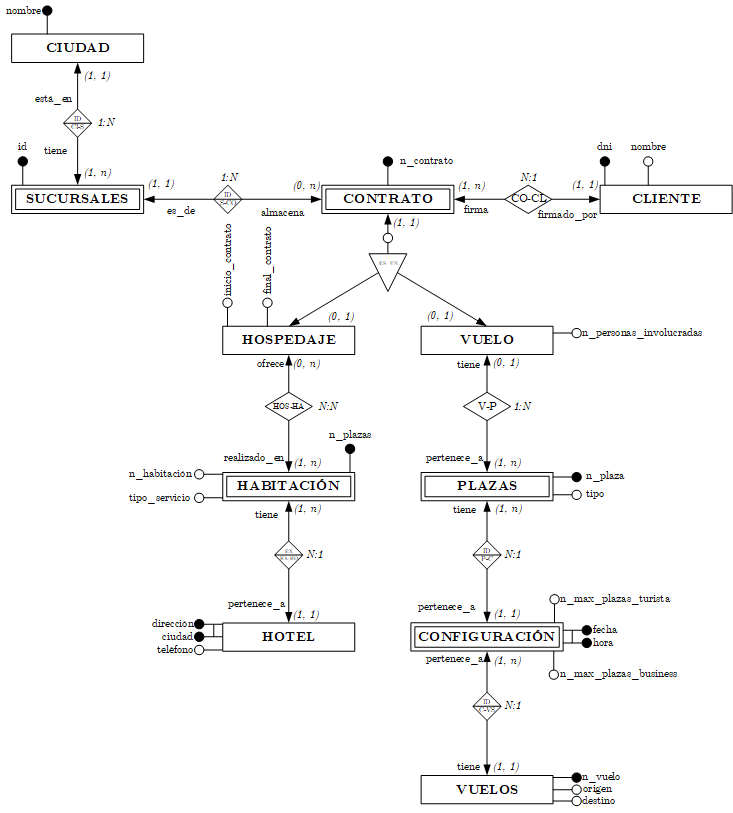
\includegraphics[scale=.63, angle=0]{img/er.png}\\
\end{centering}

\pagebreak
\section{Modelo Relacional}
\begin{centering}
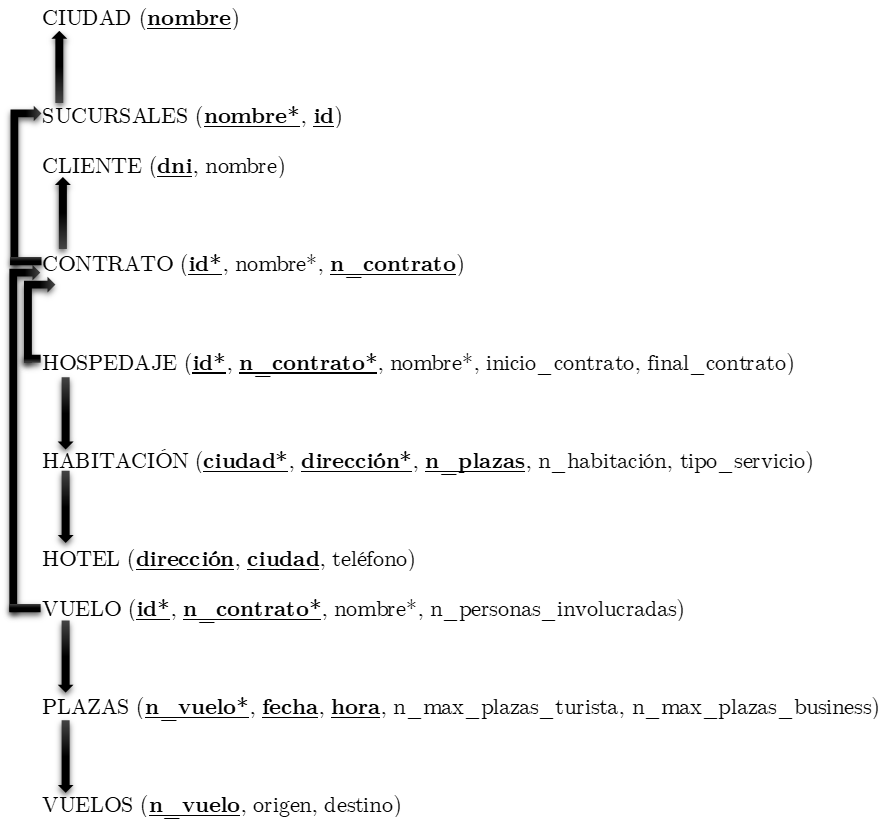
\includegraphics[scale=.63, angle=0]{img/r.png}\\
\end{centering}
\paragraph{}
Donde, en la tabla contrato, el tipo podrá ser hospedaje, vuelo o hospedaje+vuelo, dependiendo del valor que tome éste, se tendrá que insertar una tabla en hospedaje o vuelo, correspondientemente.

\paragraph{}
Se considera que los vuelos son un recorrido, el cual se realiza varias veces, y que cada viaje lo realiza con una configuración única.


\end{document}
